\documentclass{article}
\usepackage[utf8]{inputenc}
\usepackage{amsmath}
\usepackage{graphicx}
\usepackage[a4paper, total={6in, 10in}]{geometry}
\usepackage{float}
\usepackage{caption}
\usepackage{hyperref}
\usepackage{subcaption}
\newcommand{\xdashrightarrow}[2][]{\ext@arrow 0359\rightarrowfill@@{#1}{#2}}
\usepackage{comment}

\title{Big data 2}
\author{Anton Rosenberg}
\date{May 2022}

\begin{document}

\maketitle
\newpage
\section{a}
\subsection{Results}
\subsection{Conclusions}
\begin{table}[H]
    \centering
    \begin{tabular}{c|c|c|c|c|c}
        Number noisy pics &    \\
       Noise level  & \\
       Score \\
       Std \\
       Precentage noise in errors
    \end{tabular}
    \caption{Caption}
    \label{tab:my_label}
\end{table}
\begin{figure}[H]
\begin{subfigure}{.33\textwidth}
  \centering
  % include first image
  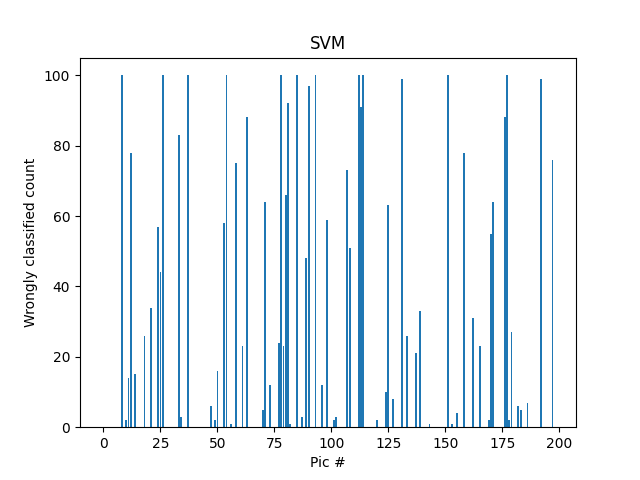
\includegraphics[width=1\linewidth]{1a/SVM.png}  
  \caption{Put your sub-caption here}
  \label{fig:sub-first}
\end{subfigure}
\begin{subfigure}{.33\textwidth}
  \centering
  % include second image
  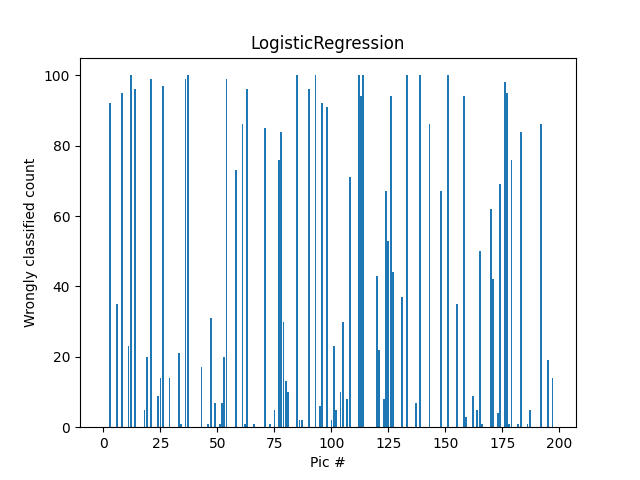
\includegraphics[width=1\linewidth]{1a/Logistic regression.png}  
  \caption{Put your sub-caption here}
  \label{fig:sub-second}
\end{subfigure}
\begin{subfigure}{.33\textwidth}
  \centering
  % include second image
  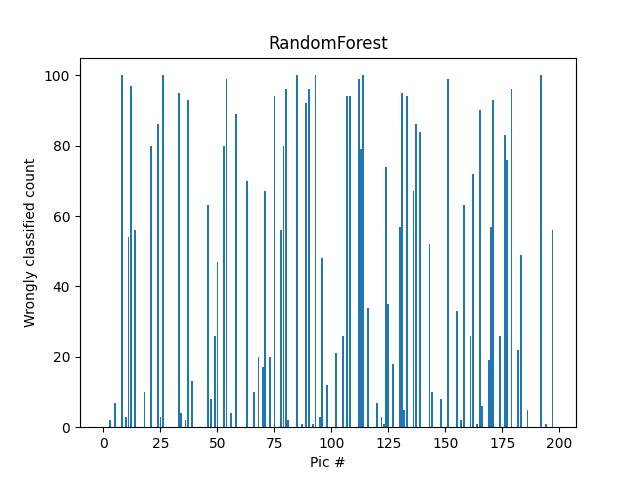
\includegraphics[width=1\linewidth]{1a/Random Forest.png}  
  \caption{Put your sub-caption here}
  \label{fig:sub-second}
\end{subfigure}
\caption{Put your caption here}
\label{wrong}
\end{figure}
\begin{figure}[H]
    \centering
    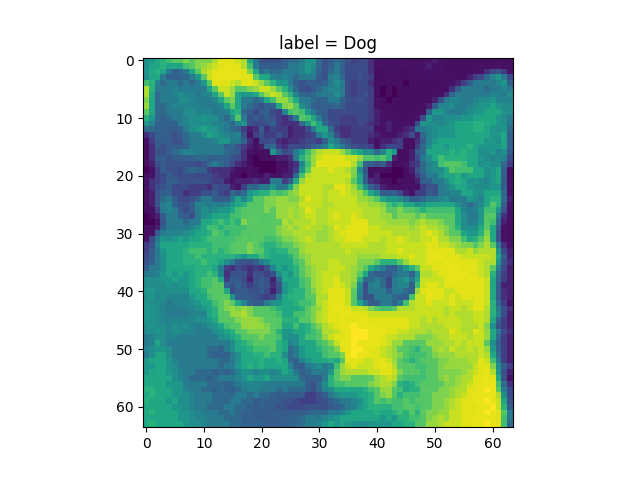
\includegraphics[scale=0.5]{1a/Dirty data.png}
    \caption{Faulty data}
    \label{faulty data}
\end{figure}
\end{document}